\documentclass[a4paper,11pt]{article}

/stock/16_git_repo/library/library.tex

\begin{document}

On cherche à optimiser plusieurs critères en même temps.
\begin{ex}
    On veut acheter un vélo et on cherche à minimiser le poids et le coût du vélo.
    \begin{figure}
        \begin{center}
            \begin{tikzpicture}[>=latex, scale=0.4]
                \draw[->] (0,0) to (0, 22);
                \draw[->] (0,0) to (25, 0);
                
                \node at (0, 23) {prix ($\times 100$\euro)};
                \node at (27, -2) {poids (kg)};
                
                \draw[-] (-0.3, 10) -- (0.3, 10);
                \draw[-] (-0.3, 20) -- (0.3, 20);

                \draw[-] (10, -0.3) -- (10, 0.3);
                \draw[-] (20, -0.3) -- (20, 0.3);

                \node at (-1, -1) {$0$};
                \node at (-1, 10) {$10$};
                \node at (-1, 20) {$20$};

                \node at (10, -1) {$10$};
                \node at (20, -1) {$20$};

                \node[label={$c(5, 18)$}] at (5, 18) {$\bullet$};
                \node[label={$d(13, 16)$}] at (13, 16) {$\bullet$};
                \node[label={$a(18, 4)$}, purple] at (18, 4) {$\bullet$};
                \node[label={$e(5, 15)$}, purple] at (5, 15) {$\bullet$};
                \node[label={$b(12, 12)$}, purple] at (12, 12) {$\bullet$};

                \draw[-, purple, thick] (18, 0) -- (18, 4) -- (0, 4);
                \draw[-, purple, thick] (5, 0) -- (5, 15) -- (0, 15);
                \draw[-, purple, thick] (12, 0) -- (12, 12) -- (0, 12);

            \end{tikzpicture}
        \end{center}
    \end{figure}
\end{ex}

\begin{df}
    On dit qu'une solution $a$ domine une solution $b$ si et seulement si $\Obj_i(a) \leq \Obj_i(b) \quad
    \forall i$ et il existe $j$ tel que $\Obj_j(a) < \Obj_j(b)$
\end{df}

\begin{df}
    Les données non dominées sont dites efficaces et appelées \emph{optima de Pareto}.
\end{df}

\begin{df}
    Une solution efficace qui petu être trouvée en optimisant une combinaison linéaire des objectifs
    est dite \emph{supportée}.
\end{df}

\begin{rq}
    Il existe des optima de Pareto non supportés.
\end{rq}

\subsection{Plus court chemin bicritère}

Soit $G=(V, E)$ un graphe avec $V = (v_0, \dots, v_n)$ tel que : $\forall 0 \leq i < n$ il y a $2$
arêtes de $v_i$ à $v_{i+1}$ de poids $(2^i, 0)$ et $(0, 2^i)$.

%fig 2

On cherche le plus court chemin bicritère de $v_0$ à $v_n$.
\begin{figure}
    \begin{center}
        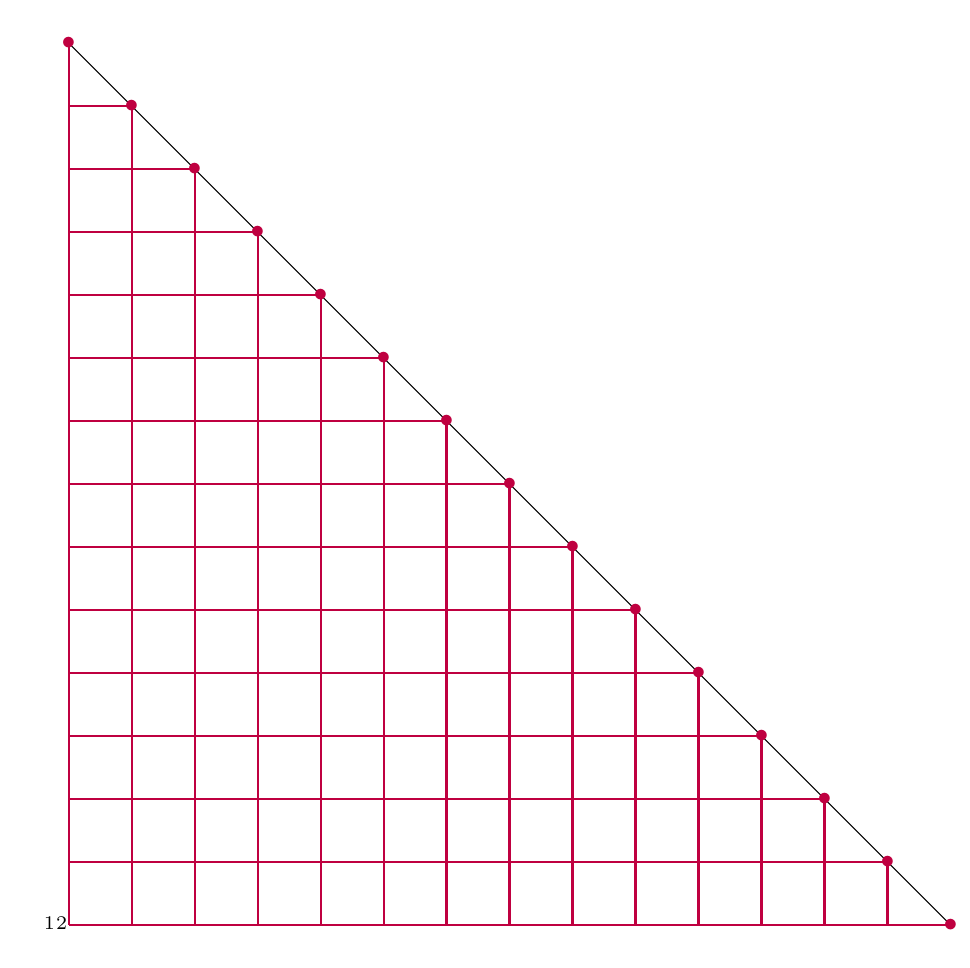
\begin{tikzpicture}[scale=0.8]
            \base{15}{15}{$\Obj_1$}{$\Obj_2$};

            \draw[-] (14, 0) -- (0, 14);
            \foreach \x [evaluate=\x as \y using 14 - \x]in {0,1,2,3,4,5,6,7,8,9,10,11,12,13,14} {
                \node[purple] at (\x, \y) {$\bullet$};
                \draw[-, thick, purple] (\x, 0) -- (\x, \y) -- (0, \y);
            }
        \end{tikzpicture}
    \end{center}
\end{figure}

Pour toutes les solutions, la somme des poids des $2$ critères est $2^n -1$ il y a donc un nombre
exponentiel d'optima de Pareto.

\begin{df}
    Une solution $s$ est $\epsilon-$approchée si pour toute solution réalisable $s$, 
    \begin{displaymath}
        \Obj(s) \leq (1 + \epsilon) \Obj(s')
    \end{displaymath}
\end{df}

\begin{df}
    On définit une relation d'$\epsilon-$dominance :
    \begin{displaymath}
        %fig 3
    \end{displaymath}
\end{df}

% Courbe de pareto

% fig 4

\begin{thrm}[Papadimitriou et Yannabarbès]
    Pour tout problème multi-objectif et pour tout $\epsilon > 0$, il existe une
    $\epsilon-$approximation de taille polynomiale en $|I|$ et $\frac{1}{\epsilon}$
\end{thrm}

\subsection{Coupe maximale pondérée bicritère}

\textbf{Données :} Un graphe $G=(V, E)$ un poids $w_{ij}$ et une longueur $l_{ij}$ pour toute arête
$(i, j) \in E$\\
\textbf{Résultat :} Une partition $(S, \overline{S})$ des sommets\\
\textbf{Objectif :} Maximiser le poids total $W(S, \overline{S}) = \sum_{i \in S, j \in
\overline{S}} w_{ij}$ ET la longueur totale $L(S, \overline{S})$.

Supposons un algorithme $\lambda-$approché pour le problème MAXCUT connu.

\begin{algorithm}[h]
    \caption{COUPE BICRITERE}
    \begin{algorithmic}[1]
        \State Calculer une coupe $(S_1, \overline{S_1})$ telle que $W(S_1, \overline{S_1}) \geq
        \lambda OPT(W)$
        \State Calculer une coupe $(S_2, \overline{S_2})$ telle que $L(S_2, \overline{S_2}) \geq
        \lambda OPT(L)$
        \State Soit $(S_3, \overline{S_3})$ la coupe telle que $S_3 = (S_1 \cap S_2) \cup
        (\overline{S_1} \cap \overline{S_2})$
        \If{$L(S_1, \overline{S_1}) \geq 0,5 L(S_2, \overline{S_2})$}
            \State Retourner $(S_1, \overline{S_1})$
        \ElsIf{$W(S_2, \overline{S_2}) \geq 0,5 W(S_1, \overline{S_1})$}
            \State Retourner $(S_2, \overline{S_2})$
        \Else
            \State Retourner $(S_3, \overline{S_3})$
        \EndIf
    \end{algorithmic}
\end{algorithm}

% figure 5

\begin{itemize}
    \item* Cas 1 $\rightarrow$ OK
    \item* Cas 2 $\rightarrow$ OK
    \item* Cas 3 : Soit 
        $E_1 = (S_1, \overline{S_1}) - (S_2, \overline{S_2})$ %vert
        $E_2 = (S_2, \overline{S_2}) - (S_1, \overline{S_1})$ %rouge
        $E_3 = (S_1, \overline{S_1}) \cap (S_2, \overline{S_2})$ %bleu
        Alors $L(E_1) + L(E_3) < 0,5(L(E_2) + L(E_3))$ donc $L(E_3) < L(E_2)$ donc $0,5(L(E_2) +
        L(E_3)) < L(E_2) < L(E_2) + L(E_1)$. On a donc $(S_3, \overline{S_3})$ est une
        $\frac{\lambda}{2} -$approximation pour $L$.
\end{itemize}

\chapter{Marin}

\begin{df}
    Etant donné une instance $I$ d'un problème multi objectif, la valeur $z(I)$ (zénith = $z_1,
    \dots, z_k$) est le \emph{minimum sur toutes les coordonnées séparées}.
\end{df}

\begin{rq}
    Il n'existe pas toujours une solution faisable de valeur $z(I)$.
\end{rq}

\begin{df}
    $S = (S_1, \dots, S_x)$ est une $\rho = (\rho_1, \dots, \rho_r)$ approximation zénith si et
    seulement si : \begin{displaymath}
        \forall i, S_i \leq \rho_i z_i
    \end{displaymath}
\end{df}

\begin{ex}
    On prend $P||(\sum c_i, C_{max})$, qui est intéressant à priori car pour minimiser $\sum c_i$,
    on veut ordonnancer les petites tâches d'abord alors que pour $C_{max}$ on ptivilégiera plutot
    les grandes tâches d'abord.

    \begin{enumerate}
        \item \textbf{Une $(1,2)-$approx zenith triviale :}\\

            $SPT$ est une $(1, 2)-$approx zénith car $SPT$ est optimale pour $\sum c_i$ et $SPT$ est
            un algo de type liste scheduling, il s'agit donc d'une $2-$approx pour $C_{max}$.
        \item \textbf{Une $(1 + \alpha, 1 + \frac{1}{\alpha})$approx zénith :}\\

            Soit $A_{C_{max}}$ un algo pour $C_{max}$ de ration $\rho_{C_{max}}$.
            Soit $A_{\sum c_i}$ un algo pour $\sum c_i$ de ration $\rho_{\sum c}$.

            On va mélanger les $2$ algorithmes.

            %fig 6
            
            % Algo 1

    \end{enumerate}
\end{ex}

\end{document}
